\section{Locating roots}
\subsection{Method}
If a function $f(x)$ is continuous on the interval $[a,b]$ and $f(a)$ and $f(b)$ have opposite signs, then $f(x)$ has at least one root, $x$, which satisfies $a<x<b$
\subsection{How change of sign can fail}
\begin{itemize}
    \item When the interval is too large sign may not change as there may be an even number of roots
    \item If the function is not continuous, sign may change but there may be an asymptote e.g. reciprocal graph
\end{itemize}

\subsection{Model answer}
\begin{itemize}
    \item $f\left( a \right) = \dots$
    \item $f\left( b \right) = \dots$
    \item There is a change of sign in the interval $[a, b]$ and $f\left( x \right)$ is continuous so there is at least one root in this interval
\end{itemize}

\section{Iteration diagrams}
\subsection{Convergent diagrams}
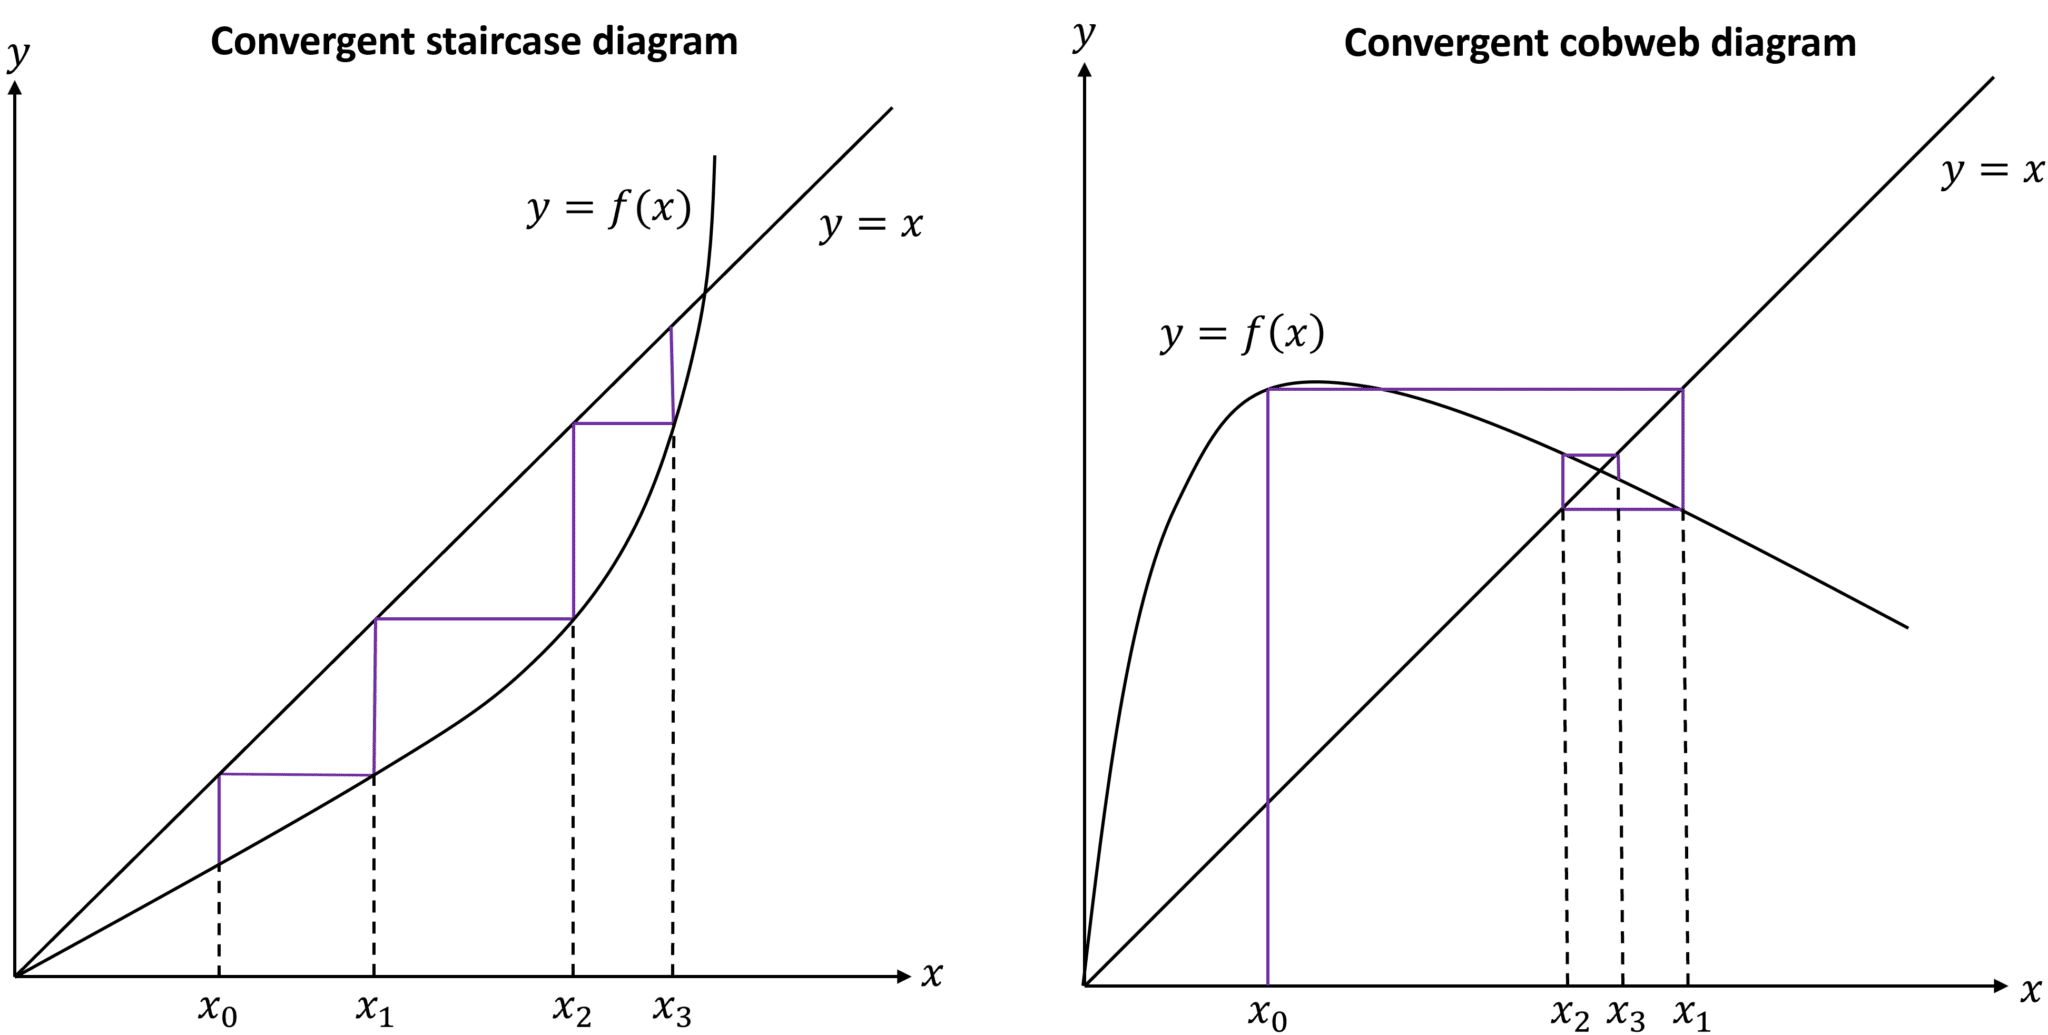
\includegraphics[width=\linewidth]{Cobwebstaircase.png}
\subsection{Divergent diagrams}
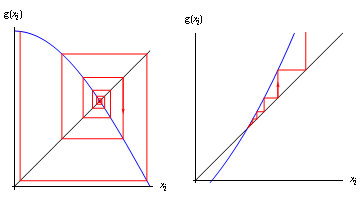
\includegraphics[width=0.6\linewidth]{fixed_point_iteration_im3.png}